% para incluir python, las siguientes fuentes:
% https://ctan.org/pkg/pythontex
% https://tug.org/tug2013/slides/Mertz-A_Gentle_Introduction_to_PythonTeX.pdf
% https://www.12000.org/my_notes/python_in_latex/index.htm

%\chapterimage{chapter_head_1.pdf} % Chapter heading image
\chapter{Introducción}
\label{chap:intro}

\section{Motivación del proyecto}
\label{sec:resumen}
% # Resumen: Motivación del proyecto

\lipsum[1-1]~\cite{Karabati2009, Letham:2016}. % Dummy text

\begin{remark}\textbf{\lipsum[1-1]}\end{remark} 

\lipsum[1-1] \footnote{Datos \emph{anonimizados} significa que no se conoce (ni se puede inferir) la identidad de los usuarios. Utilizando un número opaco para identificar a cada usuario (sin significado en la realidad).}.

\lipsum[1-1] % Dummy text.


\section{Resumen ejecutivo}
\label{sec:ejecutivo}

\subsubsection{Sobre las fuentes de información.}
\lipsum[1-2] % Dummy text

\subsubsection{Sobre los objetivos y resultados.}

\lipsum[1-3] % Dummy text






%\chapterimage{chapter_head_1.pdf} % Chapter heading image
\chapter{Contexto}
\label{chap:contexto}

\lipsum[1-2] % Dummy text


\section{Los terminales móviles}
\label{sec:terminales}

\lipsum[1-3] % Dummy text
Tabla~\ref{tab:marcas_top} y Figura~\ref{fig:marcas}.


% latex table generated in R 3.4.2 by xtable 1.8-2 package
% Fri Dec  1 13:42:06 2017
\begin{table}[ht]
\centering
\begin{tabular}{lr}
  \hline
marca & ventas \\ 
  \hline
samsung & 16 \\ 
  lgelectronics & 6 \\ 
  alcatel & 2 \\ 
  apple & 2 \\ 
  nokia & 2 \\ 
  huawei & 1 \\ 
  sony & 1 \\ 
   \hline
\end{tabular}
\caption{Cantidad de venta para las principales marcas en el período de estudio.} 
\label{tab:marcas_top}
\end{table}


\begin{figure}[bhtp]
\begin{center}
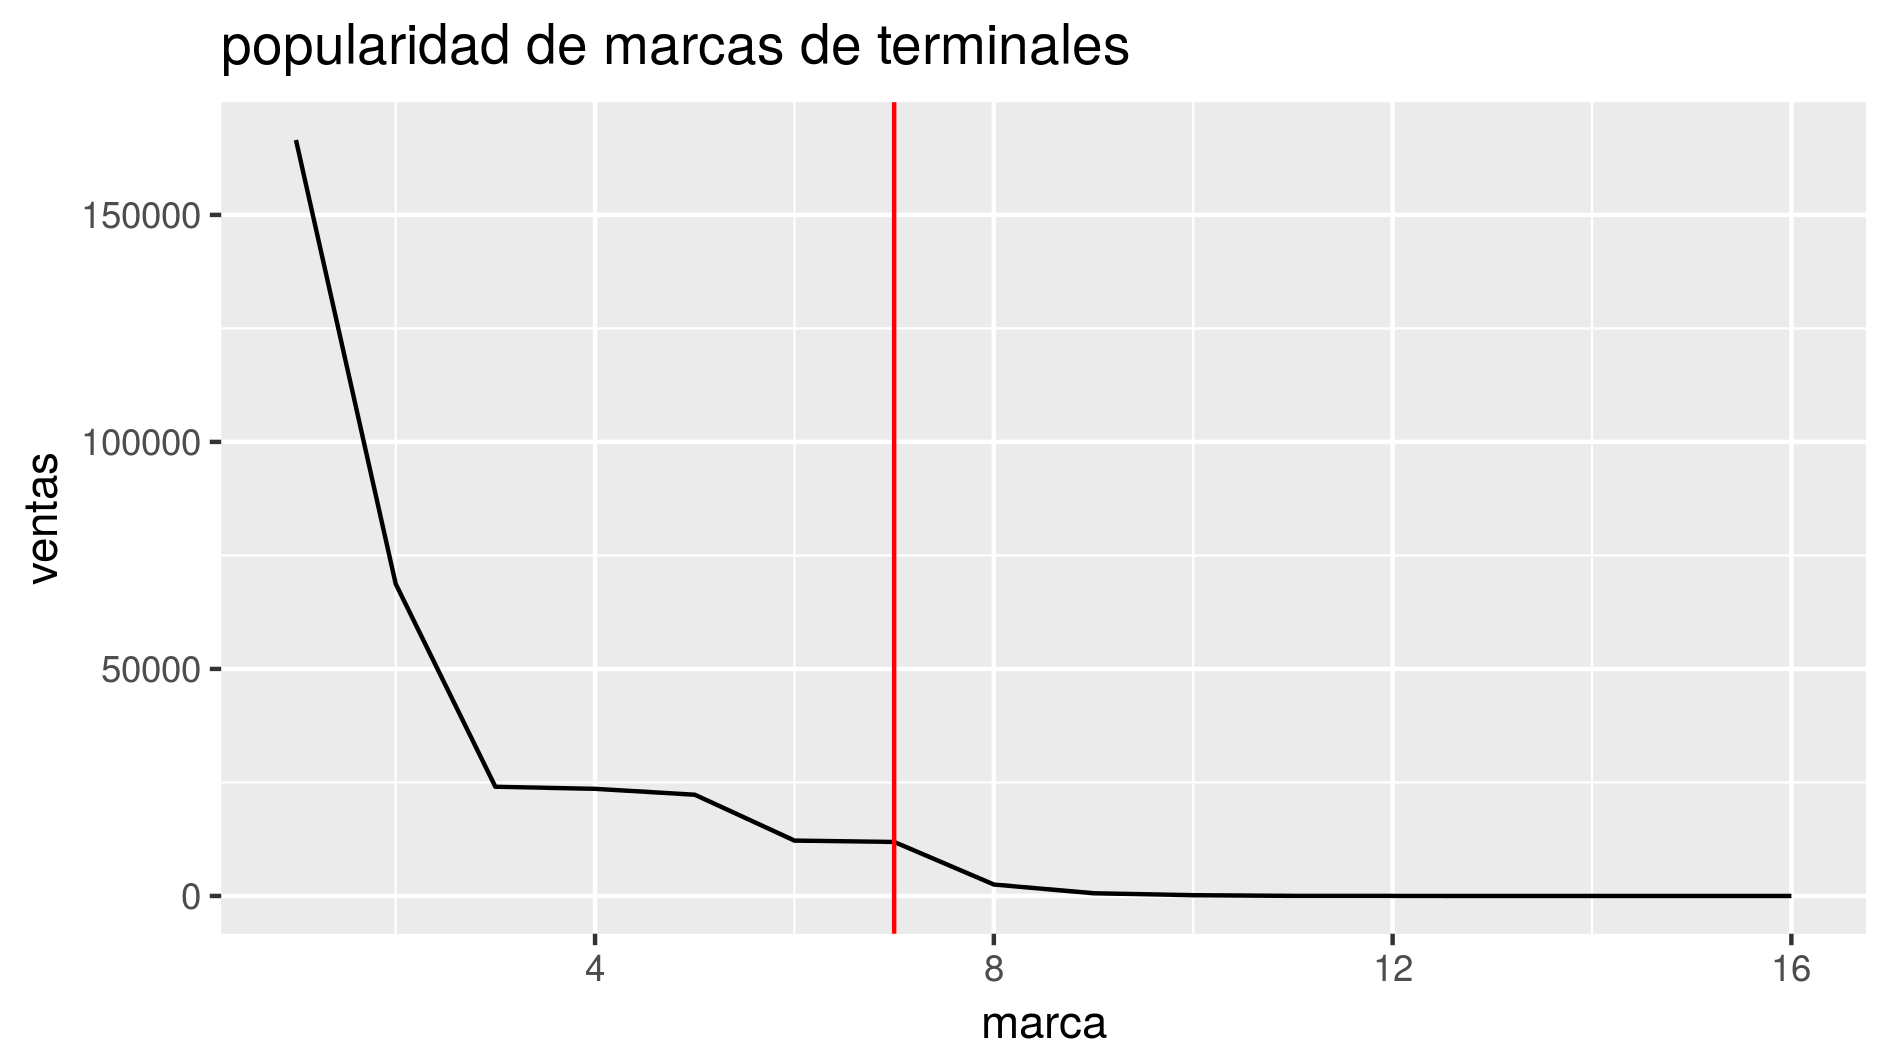
\includegraphics[scale=0.6]{figures/ejemplo.png}
\caption{Cantidad de ventas por marca. Separando con la linea roja las principales marcas del resto.}
\label{fig:marcas}
\end{center}
\end{figure}



\begin{pycode}
from pylab import *

# Define f(t), the desired function to plot
def f(t):
    return cos(2 * pi * t) * exp(-t)

# Generate the points (t_i, y_i) to plot
t = linspace(0, 5, 500)
y = f(t)

# Begin with an empty plot, 5 x 3 inches
clf()
figure(figsize=(5, 3))

# Use TeX fonts
rc("text", usetex=True)

# Generate the plot with annotations
plot(t, y)
title("Damped exponential decay")
text(3, 0.15, r"$y = \cos(2 \pi t) e^{-t}$")
xlabel("time (s)")
ylabel("voltage (mV)")

# Save the plot as a PDF file
savefig("figures/ejemplopy.pdf", bbox_inches="tight")

# Include the plot in the current LaTeX document
print(r"\begin{figure}[bhtp]\begin{center}")
print(r"\includegraphics[width=0.65\textwidth]{figures/ejemplopy.pdf}")
print(r"\caption{Generada on the fly.}\label{fig:onthefly}")
print(r"\end{center}\end{figure}")
\end{pycode}


